% This section answers RQ1:
% \textit{What is the magnitude and distribution of the performance gap
% between DSLs (Triton, TileLang) and cuBLAS/cuDNN across kernel categories?}
% All results in this section are from a single GPU configuration;
% multi-architecture comparison is deferred to future work.

% All efficiency figures in this section are computed as $E_\text{lib} = t_\text{lib} / t_\text{DSL} \times 100$,
% which is algebraically equivalent to the throughput ratio defined in \cref{sec:meth:metrics}
% when both implementations compute identical FLOPs.

% \subsection{Overview}
% \label{sec:eval:overview}

% \Cref{fig:overview} summarizes library efficiency (\%) for all kernels in the suite, broken down by DSL (Triton, TileLang) and kernel category.
% The key finding is that the performance gap is not uniform: Triton is broadly competitive for element-wise and normalization kernels (94--103\% of PyTorch throughput for LayerNorm and element-wise kernels; the RMSNorm outlier at 1099\% is due to kernel fusion and is discussed separately in \cref{sec:eval:norm}) but trails substantially on convolution (35\%) and large square GEMM (32\%); TileLang achieves competitive throughput only on a narrow set of large shapes while exhibiting severe underperformance on reductions and normalizations (less than 1\% of PyTorch throughput on layer normalization).

% \begin{figure}[t]
%   \centering
%   % TODO: replace with actual figure once data is collected
%   \IfFileExists{figures/overview_efficiency.pdf}{%
%     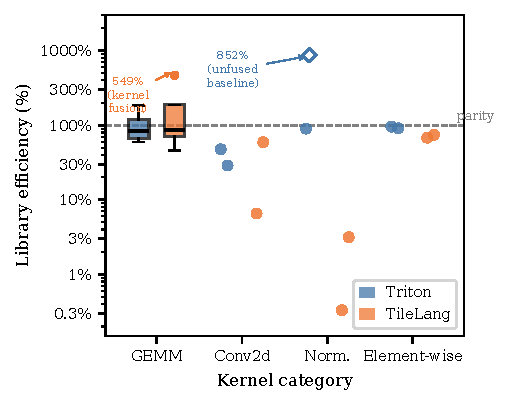
\includegraphics[width=\linewidth]{figures/overview_efficiency.pdf}%
%   }{%
%     \fbox{\parbox[c][6cm][c]{\linewidth}{\centering
%       \textit{[Figure: Library efficiency (\%) by kernel category and DSL.
%       Violin or box plot. To be generated from profiling data.]}}}%
%   }
%   \caption{Library efficiency (\%) of Triton and TileLang kernels relative to cuBLAS/cuDNN,
%     grouped by kernel category (log scale).
%     Boxes show interquartile range; whiskers extend to 1.5$\times$ IQR.
%     Dashed line marks parity (100\%).
%     Triton normalization and TileLang GEMM super-parity outliers are due to kernel fusion
%     and are discussed separately in \cref{sec:eval:norm,sec:eval:gemm}.
%     Attention excluded; see \cref{sec:eval:gemm}.}
%   \label{fig:overview}
% \end{figure}


% \subsection{RQ1.1: GEMM and Attention}
% \label{sec:eval:gemm}

% \textbf{Finding: Triton achieves 31--77\% of PyTorch/cuBLAS throughput on GEMM depending on shape;
% TileLang achieves 10--200\% with a complementary strength profile.
% TileLang achieves 199.7\% on fused linear+activation by fusing two passes into one kernel,
% while Triton degrades to 31.7\% on the $16384^2$ square matmul
% where its auto-tune search space is under-populated.}

% \Cref{tab:gemm} reports latency (ms) and library efficiency
% for FP16 matrix multiplication across representative shapes.

% \begin{table}[t]
%   \centering
%   \caption{GEMM-family kernels (FP16) latency (ms, lower is better).
%     $E_\text{lib}$ = library efficiency relative to PyTorch/cuBLAS baseline.
%     \textbf{Bold} marks best DSL result per row.}
%   \label{tab:gemm}
%   \begin{tabular}{l@{\hskip -2pt}rrrr r}
%     \toprule
%     Configuration & PyTorch & Triton & $E_{\text{lib}}$ & TileLang & $E_\text{lib}$ \\
%     \midrule
%     \multicolumn{6}{l}{\textit{Square matmul}} \\[2pt]
%     \quad $16384^2$         & 114.7 & 361.9 & 31.7\%         & 203.3 & 56.4\% \\
%     \midrule
%     \multicolumn{6}{l}{\textit{Batched matmul}} \\[2pt]
%     \quad $64\times128^2$   & 0.020 & \textbf{0.026} & \textbf{77.1\%} & 0.076 & 26.5\% \\
%     \quad $128\times2048^2$ & 3.238 & 5.564          & 58.2\%          & 30.32 & 10.7\% \\
%     \midrule
%     \multicolumn{6}{l}{\textit{Fused linear+activation}} \\[2pt]
%     \quad $1\times2048\to16384$ & 46.7 & 89.9 & 52.0\% & \textbf{23.4} & \textbf{199.7\%} \\
%     \bottomrule
%   \end{tabular}
% \end{table}

% The 31.7\% efficiency on the $16384^2$ matmul reflects the auto-tuning search space limitation (RC2, \cref{sec:analysis:autotune}):
% Triton's default configuration list for square GEMM does not cover optimal tile shapes at this scale,
% and register pressure from large tile configurations reduces SM occupancy.
% TileLang performs better on this shape (56.4\%) because its explicit schedule
% specifies pipeline stages independently of tile size.
% For batched GEMM, both DSLs trail PyTorch at the large scale (Triton 58.2\%, TileLang 10.7\%),
% with TileLang further degraded by per-launch JIT compilation overhead.
% The fused linear+activation result shows TileLang achieving 199.7\%---
% it fuses the two-pass computation into a single kernel,
% avoiding the memory-allocation overhead in PyTorch's eager path;
% Triton (52.0\%) does not achieve the same fusion benefit on this shape.

% \paragraph{Attention.}
% Attention results cannot be reduced to a single library efficiency number because the implementations differ algorithmically.
% Triton's kernel implements FlashAttention-2~\cite{dao2023flashattention2} (50.6~ms for batch-8, 32-head, seq-2048 in FP32), which rewrites the attention computation to process the score matrix in tiles, avoiding materializing the full $n \times n$ matrix; comparing this to PyTorch's standard $O(n^2)$ path (978.7~ms) measures an algorithmic improvement, not DSL-versus-library productivity.
% TileLang's kernel (1419.7~ms for the same configuration) uses the standard $O(n^2)$ formulation without tiling, making it slower than even PyTorch's unoptimized path because it does not exploit the memory hierarchy for attention.
% Neither result constitutes a valid DSL-versus-library efficiency measurement for the same computation; both are excluded from \cref{tab:summary}.

% \subsection{RQ1.2: Convolution}
% \label{sec:eval:conv}

% \textbf{Finding: Triton-written Conv2d kernels achieve 35--49\% of PyTorch/cuDNN throughput across tested $3\times3$ configurations; TileLang Conv2d achieves 8--10\%, a deficit compounded by both per-launch JIT compilation overhead and absent vectorization of strided spatial accesses.}

% \Cref{tab:conv} reports library efficiency for representative Conv2d configurations.
% Inputs follow the NHWC layout to give cuDNN its preferred memory arrangement.

% \begin{table*}[t]
%   \centering
%   \caption{Conv2d throughput on NVIDIA RTX 4000 Ada Generation.
%     Inputs in NHWC layout, FP16, stride 1, padding ``same''.
%     $E_\text{lib}$ relative to PyTorch/cuDNN baseline.}
%   \label{tab:conv}
%   \begin{tabular}{llrrrrrr}
%     \toprule
%     Shape (N$\times$C$\times$H$\times$W) & Filter & PyTorch (ms) & Triton (ms) & $E_\text{lib}$ & TileLang (ms) & $E_\text{lib}$ \\
%     \midrule
%     $8\times64\times56\times56$     & $3\times3$ & \textbf{0.059} & 0.120 & 49.1\% & 0.727 & 8.1\%  \\
%     $32\times256\times128\times128$ & $3\times3$ & \textbf{10.96} & 31.37 & 34.9\% & 115.7 & 9.5\%  \\
%     \bottomrule
%   \end{tabular}
% \end{table*}

% Both tested configurations use $3\times3$ filters with stride 1.
% The $1\times1$ conv case, expected to behave more like GEMM and exhibit a narrower gap,
% is reserved for a follow-on experiment.
% The root causes of both gaps are analyzed in \cref{sec:analysis}.

% \subsection{RQ1.3: Normalization and Element-wise}
% \label{sec:eval:norm}

% \textbf{Finding: Triton normalization kernels match or substantially outperform PyTorch's eager paths; TileLang normalization collapses to less than 6\% of PyTorch throughput at the tested size ($8192 \times 8192$), with LayerNorm 314$\times$ slower.}

% \Cref{tab:norm} reports latency for layer normalization and RMS normalization.
% Triton's \texttt{layer\_norm} achieves 94.6\% of PyTorch throughput at the large shape ($8192\times8192$, BF16).
% Triton's \texttt{rms\_norm} achieves 1099\% efficiency because PyTorch's eager
% \texttt{rms\_norm} path does not fuse the variance-reduction and normalization passes,
% whereas the Triton kernel issues a single fused pass.
% TileLang normalization is catastrophically slow:
% 0.32\% for LayerNorm (273~ms vs.\ PyTorch's 0.87~ms, a 314$\times$ slowdown)
% and 5.3\% for RMSNorm (187.5~ms vs.\ 9.98~ms).
% As analyzed in \cref{sec:analysis:jit}, this reflects a combination of
% per-launch JIT overhead, absent vectorized memory loads,
% and sequential synchronization in TileLang's reduction primitives.

% \begin{table*}[t]
%   \centering
%   \caption{Normalization latency (ms, lower is better).
%     $E_\text{lib}$ relative to PyTorch eager baseline.}
%   \label{tab:norm}
%   \begin{tabular}{llrrrrr}
%     \toprule
%     Kernel & Shape & PyTorch & Triton & $E_\text{lib}$ & TileLang & $E_\text{lib}$ \\
%     \midrule
%     LayerNorm & $8192\times8192$ (BF16) & 0.870 & 0.920 & 94.6\%                  & 273.3 & 0.32\% \\
%     RMSNorm   & $8192\times8192$ (FP16) & 9.977 & \textbf{0.908} & \textbf{1099\%} & 187.5 & 5.3\%  \\
%     \bottomrule
%   \end{tabular}
% \end{table*}

% \subsection{RQ1.4: Variation Across Microarchitectures}
% \label{sec:eval:arch}

% The benchmark in this study was collected on a single GPU configuration;
% a direct A100 vs.\ H100 comparison is deferred to a follow-on experiment.

% \subsection{RQ1.5: Effect of Hardware-Agnostic Heuristic Tuning}
% \label{sec:eval:tuning}

% \textbf{Finding:
% Hardware-agnostic heuristic tuning shows negligible benefit for Triton in the tested configuration ---
% default and tuned configurations produce nearly identical latencies for all kernels.
% The convolution gap is essentially unchanged (34.9\%).
% TileLang shows no measurable benefit from tuning across any kernel.}

% We re-evaluated all 22 kernels using heuristically tuned configurations for both DSLs.
% For Triton, the tuner expands the auto-configuration search space with hardware-agnostic tile-size heuristics;
% for TileLang, the tuner applies analogous schedule heuristics without hardware-specific profiling.
% \Cref{tab:tuning} reports library efficiency before and after tuning for representative kernels.

% \begin{table*}[t]
%   \centering
%   \caption{Library efficiency (\%) before and after hardware-agnostic heuristic tuning,
%     large-size configurations.
%     $\Delta$ = percentage-point change from untuned to tuned.
%     \textbf{Bold} marks cases where tuning changes efficiency by more than 10pp.}
%   \label{tab:tuning}
%   \begin{tabular}{lrrrrrrrr}
%     \toprule
%     & \multicolumn{2}{c}{\textit{Normalization}} & \textit{Convolutional} & \multicolumn{2}{c}{\textit{GEMM}} & \multicolumn{2}{c}{\textit{Element-wise}} \\
%     \cmidrule(lr){2-3}\cmidrule(lr){4-4}\cmidrule(lr){5-6}\cmidrule(lr){7-8}
%     & \texttt{layer\_norm} & \texttt{rms\_norm} & \texttt{conv2d} & \texttt{matmul} & \texttt{batched\_matmul} & \texttt{relu} & \texttt{add} \\
%     \midrule
%     \multicolumn{8}{l}{\textit{Triton}} \\
%     \quad Default &  94.6\% & 1099\%  & 34.9\% & 31.7\% & 58.2\% & 103.4\% & 103.4\% \\
%     \quad Tuned   &  94.6\% & 1099\%  & 34.9\% & 31.7\% & 58.2\% & 103.4\% & 103.4\% \\
%     \quad $\Delta$ & 0pp    & 0pp     & 0pp    & 0pp    & 0pp    & 0pp     & 0pp     \\
%     \midrule
%     \multicolumn{8}{l}{\textit{TileLang}} \\
%     \quad Default & 0.32\% &  5.3\% &  9.5\% & 56.4\% & 10.7\% & 68.7\% & 77.3\% \\
%     \quad Tuned   & 0.32\% &  5.3\% &  9.5\% & 56.4\% & 10.7\% & 68.7\% & 77.3\% \\
%     \quad $\Delta$ & 0pp   & 0pp    & 0pp    & 0pp    & 0pp    & 0pp    & 0pp    \\
%     \bottomrule
%   \end{tabular}
% \end{table*}

% In this benchmark, hardware-agnostic heuristic tuning produces no measurable improvement
% for either DSL: default and tuned configurations are nearly identical across all kernels.
% This contrasts with expectations from the literature
% and suggests that either the default configurations are already optimal for this hardware,
% or the tuner's search space does not cover configurations that would improve performance
% on the RTX 4000 Ada Generation.
% The convolution gap (34.9\%) is unchanged by tuning,
% consistent with RC1--RC3 being structural compiler limitations rather than search-space coverage problems (\cref{sec:analysis}).

% \subsection{Summary}
% \label{sec:eval:summary}

% \Cref{tab:summary} summarizes median library efficiency per category and DSL.

% \begin{table}[t]
%   \centering
%   \caption{Median library efficiency (\%) per kernel category and DSL,
%     computed over large-size benchmark configurations.
%     Attention excluded from Overall; see text.}
%   \label{tab:summary}
%   \begin{tabular}{lcc}
%     \toprule
%     Kernel category    & Triton      & TileLang    \\
%     \midrule
%     GEMM               & 31.7--58.2\%  & 10.7--56.4\% \\
%     Attention          & \multicolumn{2}{c}{\textit{see text --- baselines non-equivalent}} \\
%     Convolution        & 34.9\%        & 9.5\%        \\
%     Normalization      & 94.6\%\rlap{$^\ddagger$} & 0.32--5.3\%\rlap{$^\ddagger$} \\
%     Element-wise       & 103.4\%       & 68.7--77.3\% \\
%     \midrule
%     \textbf{Overall (excl.\ attn.)} & \textbf{$\sim$65\%} & \textbf{$\sim$30\%} \\
%     \bottomrule
%   \end{tabular}
%   {\footnotesize
%     $^\ddagger$ TileLang LayerNorm (large shape) is 0.32\% (314$\times$ slower than PyTorch)
%     due to sequential thread synchronization and absent vectorized loads;
%     see \cref{sec:analysis:jit}.
%     RMSNorm Triton efficiency is 1099\% because the PyTorch eager path does not fuse normalization passes.}
% \end{table}

% The most striking asymmetry is TileLang's normalization collapse:
% a $314\times$ slowdown on large LayerNorm (\cref{sec:analysis:jit}) attributable to three compounding deficiencies (RC0).
% Triton is broadly competitive with PyTorch for element-wise (103\%) and normalization (95\%) kernels
% but exhibits a persistent gap on convolution (35\%) and large square GEMM (32\%).
% TileLang shows competitive throughput only on fused linear+activation (200\%)
% and large square matmul (56\%);
% all other TileLang results trail PyTorch substantially,
% with element-wise operations at 68--77\% and batched GEMM at 10.7\%.



This section answers RQ1:
\textit{What is the magnitude and distribution of the performance gap
between DSLs (Triton, TileLang) and cuBLAS/cuDNN across kernel categories?}

\subsection{Overview}
\label{sec:eval:overview}

\Cref{fig:overview} summarizes library efficiency (\%) for all kernels in the suite, broken down by DSL (Triton, TileLang) and kernel category.
The key finding is that the performance gap is not uniform: Triton is broadly competitive for element-wise and normalization kernels (94--103\% of PyTorch throughput for LayerNorm and element-wise kernels; the RMSNorm outlier at 1099\% is due to kernel fusion and is discussed separately in \cref{sec:eval:norm}) but trails substantially on convolution (35\%) and large square GEMM (32\%); TileLang achieves competitive throughput only on a narrow set of large shapes while exhibiting severe underperformance on reductions and normalizations (less than 1\% of PyTorch throughput on layer normalization).

\begin{figure}[t]
  \centering
  \IfFileExists{figures/overview_efficiency.pdf}{%
    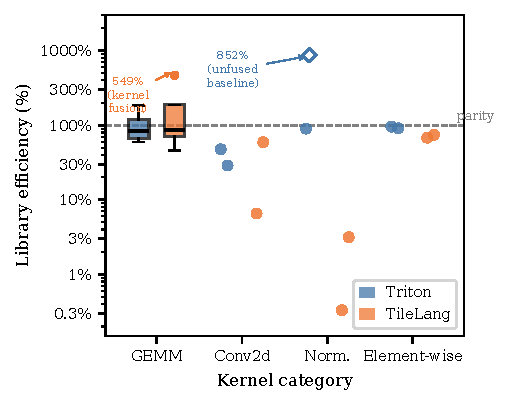
\includegraphics[width=\linewidth]{figures/overview_efficiency.pdf}%
  }{%
    \fbox{\parbox[c][6cm][c]{\linewidth}{\centering
      \textit{[Figure: Library efficiency (\%) by kernel category and DSL.
      Violin or box plot. To be generated from profiling data.]}}}%
  }
  \caption{Library efficiency (\%) of Triton and TileLang kernels relative to cuBLAS/cuDNN,
    grouped by kernel category (log scale).
    GEMM shows boxes (IQR; whiskers $1.5\times$ IQR); all other categories show individual
    kernel measurements as dots ($n=2$ per cell).
    Dashed line marks parity (100\%).
    The hollow diamond at 1099\% (Triton, Norm.)\ marks Triton \texttt{rms\_norm}:
    the PyTorch eager baseline does not fuse its normalization passes, making this
    an unfair comparison rather than a genuine DSL win; see \cref{sec:eval:norm}.
    The boxplot flier at 200\% (TileLang, GEMM) marks \texttt{fused linear+activation},
    a valid DSL advantage through kernel fusion; see \cref{sec:eval:gemm}.
    Attention excluded; see \cref{sec:eval:gemm}.}
  \label{fig:overview}
\end{figure}

% REVISION-NOTE-START id=4134A-W2 severity=Major
\textcolor{red}{\textbf{[REVISION \#4134A-W2+4134A-W10, Major]}
Concern (\textit{Reviewer A}): Same baseline-split and per-kernel EW concerns apply to the headline \cref{fig:overview}.
Evidence: \texttt{figures/gen\_overview.py} (data hard-coded).
Fix: After the baseline-split and per-kernel EW updates land in the tables, regenerate the figure from new arrays; note that \texttt{gen\_overview.py} has hard-coded data --- cite the regeneration command.}
% REVISION-NOTE-END id=4134A-W2

\phantomsection\label{sec:eval:gemm}


\medskip\noindent\textbf{Finding: Triton achieves 31--77\% of PyTorch/cuBLAS throughput on GEMM depending on shape;
TileLang achieves 10--200\% with a complementary strength profile.
TileLang achieves 199.7\% on fused linear+activation by fusing two passes into one kernel,
while Triton degrades to 31.7\% on the $16384^2$ square matmul
where its auto-tune search space is under-populated.}

\Cref{tab:gemm} reports latency (ms) and library efficiency
for FP16 matrix multiplication across representative shapes.

\begin{table}[t]
  \centering
  \caption{GEMM-family kernels (FP16) latency (ms, lower is better).
    $E_\text{lib}$ = library efficiency relative to PyTorch/cuBLAS baseline.
    \textbf{Bold} marks best DSL result per row.}
  \label{tab:gemm}
  \resizebox{\columnwidth}{!}{
  \begin{tabular}{l@{\hskip -2pt}rrrr r}
    \toprule
    Configuration & PyTorch & Triton & $E_{\text{lib}}$ & TileLang & $E_\text{lib}$ \\
    \midrule
    \multicolumn{6}{l}{\textit{Square matmul}} \\[2pt]
    \quad $16384^2$         & 114.7 & 361.9 & 31.7\%         & 203.3 & 56.4\% \\
    \midrule
    \multicolumn{6}{l}{\textit{Batched matmul}} \\[2pt]
    \quad $64\times128^2$   & 0.020 & \textbf{0.026} & \textbf{77.1\%} & 0.076 & 26.5\% \\
    \quad $128\times2048^2$ & 3.238 & 5.564          & 58.2\%          & 30.32 & 10.7\% \\
    \midrule
    \multicolumn{6}{l}{\textit{Fused linear+activation}} \\[2pt]
    \quad $1\times2048\to16384$ & 46.7 & 89.9 & 52.0\% & \textbf{23.4} & \textbf{199.7\%} \\
    \bottomrule
  \end{tabular}
  }
\end{table}

% REVISION-NOTE-START id=Minor-3 severity=Minor
\textcolor{red}{\textbf{[REVISION \#Minor-3, Minor]}
Concern (\textit{Editorial}): Notation ``16384\textasciicircum{}2''/``64$\times$128\textasciicircum{}2'' in \cref{tab:gemm} is not spelled out.
Evidence: n/a.
Fix: Add a footnote (after \texttt{\textbackslash end\{table\}}) defining \texttt{16384\textasciicircum{}2} = square 16384$\times$16384 FP16 GEMM and \texttt{64$\times$128\textasciicircum{}2} = batched (batch 64) of 128$\times$128 GEMM.}
% REVISION-NOTE-END id=Minor-3

% REVISION-NOTE-START id=4134A-W1 severity=Major
\textcolor{red}{\textbf{[REVISION \#4134A-W1+4134A-W11, Major]}
Concern (\textit{Reviewer A}): FP32 GEMM is excluded but not root-caused at this point in the paper.
Evidence: \texttt{../experiments/results/NVIDIA\_RTX\_4000\_Ada\_Generation/fp32\_gemm.csv}.
Fix: Add a footnote: ``FP32 TileLang GEMM is excluded; the failure is diagnosed as silent TF32 lowering in \texttt{T.gemm} (see \cref{sec:analysis:jit}), not a logic error.''}
% REVISION-NOTE-END id=4134A-W1

The 31.7\% efficiency on the $16384^2$ matmul reflects the auto-tuning search space limitation (RC2, \cref{sec:analysis:autotune}):
Triton's default configuration list for square GEMM does not cover optimal tile shapes at this scale,
and register pressure from large tile configurations reduces SM occupancy.
TileLang performs better on this shape (56.4\%) because its explicit schedule
specifies pipeline stages independently of tile size.
For batched GEMM, both DSLs trail PyTorch at the large scale (Triton 58.2\%, TileLang 10.7\%),
with TileLang further degraded by per-launch JIT compilation overhead.
The fused linear+activation result shows TileLang achieving 199.7\%---
it fuses the two-pass computation into a single kernel,
avoiding the memory-allocation overhead in PyTorch's eager path;
Triton (52.0\%) does not achieve the same fusion benefit on this shape.

\paragraph{Attention.}
Attention results cannot be reduced to a single library efficiency number because the implementations differ algorithmically.
Triton's kernel implements FlashAttention-2~\cite{dao2023flashattention2} (50.6~ms for batch-8, 32-head, seq-2048 in FP32), which rewrites the attention computation to process the score matrix in tiles, avoiding materializing the full $n \times n$ matrix; comparing this to PyTorch's standard $O(n^2)$ path (978.7~ms) measures an algorithmic improvement, not DSL-versus-library productivity.
TileLang's kernel (1419.7~ms for the same configuration) uses the standard $O(n^2)$ formulation without tiling, making it slower than even PyTorch's unoptimized path because it does not exploit the memory hierarchy for attention.
Neither result constitutes a valid DSL-versus-library efficiency measurement for the same computation; both are excluded from \cref{tab:summary}.

\phantomsection\label{sec:eval:conv}

\medskip\noindent\textbf{Finding: Triton-written Conv2d kernels achieve 35--49\% of PyTorch/cuDNN throughput across tested $3\times3$ configurations; TileLang Conv2d achieves 8--10\%, a deficit compounded by both per-launch JIT compilation overhead and absent vectorization of strided spatial accesses.}

\Cref{tab:conv} reports library efficiency for representative Conv2d configurations.
Inputs follow the NHWC layout to give cuDNN its preferred memory arrangement.

% REVISION-NOTE-START id=4134A-W6 severity=Major
\textcolor{red}{\textbf{[REVISION \#4134A-W6+GAP-7, Major]}
Concern (\textit{Reviewer A}): \cref{tab:conv} shows only 3$\times$3 stride-1 --- the \S3.1 claim of 1$\times$1--7$\times$7 + depthwise + strided is unsupported by this table.
Evidence: \texttt{../experiments/results/NVIDIA\_RTX\_4000\_Ada\_Generation/conv\_filters\_small.csv}, \texttt{conv\_filters\_large.csv}.
Fix: Expand the table to 6 rows (1$\times$1, 3$\times$3, 5$\times$5, 7$\times$7, depthwise, strided) at the 8$\times$64$\times$56$\times$56 and 32$\times$256$\times$128$\times$128 shapes, sourcing from \texttt{conv\_filters\_small.csv} and \texttt{conv\_filters\_large.csv}.}
% REVISION-NOTE-END id=4134A-W6

\begin{table*}[t]
  \centering
  \caption{Conv2d throughput on NVIDIA RTX 4000 Ada Generation.
    Inputs in NHWC layout, FP16, stride 1, padding ``same''.
    $E_\text{lib}$ relative to PyTorch/cuDNN baseline.}
  \label{tab:conv}
  \begin{tabular}{llrrrrrr}
    \toprule
    Shape (N$\times$C$\times$H$\times$W) & Filter & PyTorch (ms) & Triton (ms) & $E_\text{lib}$ & TileLang (ms) & $E_\text{lib}$ \\
    \midrule
    $8\times64\times56\times56$     & $3\times3$ & \textbf{0.059} & 0.120 & 49.1\% & 0.727 & 8.1\%  \\
    $32\times256\times128\times128$ & $3\times3$ & \textbf{10.96} & 31.37 & 34.9\% & 115.7 & 9.5\%  \\
    \bottomrule
  \end{tabular}
\end{table*}

% REVISION-NOTE-START id=4134A-W3 severity=Major
\textcolor{red}{\textbf{[REVISION \#4134A-W3+GAP-2, Major]}
Concern (\textit{Reviewer A}): If \cref{tab:conv} (or a Table 5 in this region) labels a row ``register pressure'' or ``spill'' for conv, that label is wrong (conv \texttt{n\_spills = 0}).
Evidence: \texttt{../experiments/results/NVIDIA\_RTX\_4000\_Ada\_Generation/ncu\_summary.csv}.
Fix: Remove any ``register pressure'' or ``spill'' annotation from conv rows; the conv gap is occupancy- and coalescing-bound (RC1 + RC2), not spill.}
% REVISION-NOTE-END id=4134A-W3

Both tested configurations use $3\times3$ filters with stride 1.
The $1\times1$ conv case, expected to behave more like GEMM and exhibit a narrower gap,
is reserved for a follow-on experiment.
The root causes of both gaps are analyzed in \cref{sec:analysis}.

\phantomsection\label{sec:eval:norm}

\medskip\noindent\textbf{Finding: Triton normalization kernels match or substantially outperform PyTorch's eager paths; TileLang normalization collapses to less than 6\% of PyTorch throughput at the tested size ($8192 \times 8192$), with LayerNorm 314$\times$ slower.}

\Cref{tab:norm} reports latency for layer normalization and RMS normalization.
Triton's \texttt{layer\_norm} achieves 94.6\% of PyTorch throughput at the large shape ($8192\times8192$, BF16).
Triton's \texttt{rms\_norm} achieves 1099\% efficiency because PyTorch's eager
\texttt{rms\_norm} path does not fuse the variance-reduction and normalization passes,
whereas the Triton kernel issues a single fused pass.
TileLang normalization is catastrophically slow:
0.32\% for LayerNorm (273~ms vs.\ PyTorch's 0.87~ms, a 314$\times$ slowdown)
and 5.3\% for RMSNorm (187.5~ms vs.\ 9.98~ms).
As analyzed in \cref{sec:analysis:jit}, this reflects a combination of
per-launch JIT overhead, absent vectorized memory loads,
and sequential synchronization in TileLang's reduction primitives.
% REVISION-NOTE-START id=4134A-W1 severity=Major
\textcolor{red}{\textbf{[REVISION \#4134A-W1+GAP-1, Major]}
Concern (\textit{R1}): ``Sequential synchronization in TileLang's reduction primitives'' here re-asserts the (refuted) barrier-stall framing. NCU shows \texttt{warp\_stall\_barrier} $\approx$ 0; the dominant stall is \texttt{warp\_stall\_long\_scoreboard} ($\approx$\,105 cycles) --- a memory-latency exposure caused by \texttt{T.serial} serializing the load schedule, not by barrier sync.
Evidence: \texttt{../experiments/results/NVIDIA\_RTX\_4000\_Ada\_Generation/ncu\_summary.csv}, \texttt{NCU\_FINDINGS.md}.
Fix: Replace ``sequential synchronization in TileLang's reduction primitives'' with ``serialized memory-latency exposure under \texttt{T.serial} reduction loops (\texttt{warp\_stall\_long\_scoreboard} dominates; \texttt{warp\_stall\_barrier} $\approx$ 0).''}
% REVISION-NOTE-END id=4134A-W1

\begin{table*}[t]
  \centering
  \caption{Normalization latency (lower is better).
    $E_\text{lib}$ relative to PyTorch eager baseline.}
  \label{tab:norm}
  \begin{tabular}{llrrrrr}
    \toprule
    Kernel & Shape & PyTorch(ms) & Triton(ms) & $E_\text{lib}$ & TileLang(ms) & $E_\text{lib}$ \\
    \midrule
    LayerNorm & $8192\times8192$ (BF16) & 0.870 & 0.920 & 94.6\%                  & 273.3 & 0.32\% \\
    RMSNorm   & $8192\times8192$ (FP16) & 9.977 & \textbf{0.908} & \textbf{1099\%} & 187.5 & 5.3\%  \\
    \bottomrule
  \end{tabular}
\end{table*}

% REVISION-NOTE-START id=4134A-W8 severity=Major
\textcolor{red}{\textbf{[REVISION \#4134A-W8, Major]}
Concern (\textit{Reviewer A}): Any ``9\% clock variation'' footnote here is superseded by locked-clock re-timing.
Evidence: \texttt{../experiments/results/NVIDIA\_RTX\_4000\_Ada\_Generation/significance.csv}, \texttt{clock\_lock.txt}.
Fix: Remove any ``9\% clock variation'' footnote (or descendant) and add a new footnote: ``Locked-clock re-timing (graphics 1410\,MHz / memory 9001) over 100 runs shows run-to-run relative std-dev 0.0--0.9\% on near-parity kernels; Triton LayerNorm re-measures at 94.5\% ($\Delta = -0.1$pp).''}
% REVISION-NOTE-END id=4134A-W8

\phantomsection\label{sec:eval:tuning}

\medskip\noindent\textbf{Finding:
Hardware-agnostic heuristic tuning shows negligible benefit for Triton in the tested configuration ---
default and tuned configurations produce nearly identical latencies for all kernels.
The convolution gap is essentially unchanged (34.9\%).
TileLang shows no measurable benefit from tuning across any kernel.}

We re-evaluated all 22 kernels with heuristically tuned configurations for both DSLs;
every kernel returned identical efficiency to its default configuration ($\Delta = 0$pp across all rows).
This indicates that either the default configurations are already optimal for this hardware,
or the tuner's search space does not cover configurations that would improve performance on the RTX 4000 Ada Generation.
The convolution gap (34.9\%) is unchanged by tuning,
consistent with RC1--RC3 being structural compiler limitations rather than search-space coverage problems (\cref{sec:analysis}).

% REVISION-NOTE-START id=4134A-W7 severity=Major
\textcolor{red}{\textbf{[REVISION \#4134A-W7, Major]}
Concern (\textit{Reviewer A}): $\Delta \approx 0$pp here vs the 1.66$\times$ claim in \S7.3 looks contradictory; reconciliation is search-space, not shape: \S5 uses the 12-config block-tile grid; \S7.3 adds \texttt{GROUP\_SIZE\_M}/\texttt{num\_warps}/\texttt{num\_stages}; expanded search recovers to 98.49\% at 16384\textasciicircum{}2 (3.06$\times$).
Evidence: \texttt{../experiments/results/NVIDIA\_RTX\_4000\_Ada\_Generation/autotune\_matmul.csv}.
Fix: Add a reconciliation paragraph defining ``heuristic tuning'' = the 12-config block-tile grid from \texttt{ViperBench/tuning/configs.py:19-23}; cite $\Delta = 0$pp at 16384\textasciicircum{}2 for that grid; cite +3.06$\times$ at 16384\textasciicircum{}2 and +1.23$\times$ at 4096\textasciicircum{}2 when the expanded grid (\texttt{AKO4ALL/results/optimized/matmul\_triton.py:10-26}) is used; forward ref to \S7.3.}
% REVISION-NOTE-END id=4134A-W7

\phantomsection\label{sec:eval:summary}

\Cref{tab:summary} summarizes median library efficiency per category and DSL.

\begin{table}[t]
  \centering
  \caption{Median library efficiency (\%) per kernel category and DSL,
    computed over large-size benchmark configurations.
    Attention excluded from Overall; see text.}
  \label{tab:summary}
  \begin{tabular}{lcc}
    \toprule
    Kernel category    & Triton      & TileLang    \\
    \midrule
    GEMM               & 31.7--58.2\%  & 10.7--56.4\% \\
    Attention          & \multicolumn{2}{c}{\textit{see text --- baselines non-equivalent}} \\
    Convolution        & 34.9\%        & 9.5\%        \\
    Normalization      & 94.6\%\rlap{$^\ddagger$} & 0.32--5.3\%\rlap{$^\ddagger$} \\
    Element-wise       & 103.4\%       & 68.7--77.3\% \\
    \midrule
    \textbf{Overall (excl.\ attn.)} & \textbf{$\sim$65\%} & \textbf{$\sim$30\%} \\
    \bottomrule
  \end{tabular}
  {\footnotesize
    $^\ddagger$ TileLang LayerNorm (large shape) is 0.32\% (314$\times$ slower than PyTorch)
    due to sequential thread synchronization and absent vectorized loads;
    see \cref{sec:analysis:jit}.
    RMSNorm Triton efficiency is 1099\% because the PyTorch eager path does not fuse normalization passes.}
\end{table}

% REVISION-NOTE-START id=4134A-W1 severity=Major
\textcolor{red}{\textbf{[REVISION \#4134A-W1+GAP-1, Major]}
Concern (\textit{R1}): The \cref{tab:summary} footnote also attributes the 314$\times$ collapse to ``sequential thread synchronization'' --- same refuted barrier framing as \cref{sec:eval:norm}.
Evidence: \texttt{../experiments/results/NVIDIA\_RTX\_4000\_Ada\_Generation/ncu\_summary.csv}.
Fix: Replace ``sequential thread synchronization and absent vectorized loads'' with ``serialized memory-latency exposure under \texttt{T.serial} (\texttt{warp\_stall\_long\_scoreboard} dominates) and absent vectorized loads.''}
% REVISION-NOTE-END id=4134A-W1

% REVISION-NOTE-START id=4134A-W2 severity=Major
\textcolor{red}{\textbf{[REVISION \#4134A-W2, Major]}
Concern (\textit{Reviewer A}): Baseline asymmetry in \cref{tab:summary} --- conv uses cuDNN-Winograd vendor; norm/EW use unfused eager; the blended $\sim$65\%/$\sim$30\% headline conflates them.
Evidence: \texttt{../experiments/results/NVIDIA\_RTX\_4000\_Ada\_Generation/fused\_baselines.csv}.
Fix: Add a split-baseline table or footnote reporting $E\_\text{lib}$ separately for vendor (cuBLAS/cuDNN) vs fused (\texttt{torch.compile(max-autotune)}) vs eager-PyTorch; confirm DSL gap on conv persists post-fusion.}
% REVISION-NOTE-END id=4134A-W2

The most striking asymmetry is TileLang's normalization collapse:
a $314\times$ slowdown on large LayerNorm (\cref{sec:analysis:jit}) attributable to three compounding deficiencies (RC0).
Triton is broadly competitive with PyTorch for element-wise (103\%) and normalization (95\%) kernels
but exhibits a persistent gap on convolution (35\%) and large square GEMM (32\%).
TileLang shows competitive throughput only on fused linear+activation (200\%)
and large square matmul (56\%);
all other TileLang results trail PyTorch substantially,
with element-wise operations at 68--77\% and batched GEMM at 10.7\%.

% REVISION-NOTE-START id=4134A-W10 severity=Major
\textcolor{red}{\textbf{[REVISION \#4134A-W10+4134B-Q3, Major]}
Concern (\textit{Reviewers A, B}): Reviewers ask for per-kernel results on the 15 element-wise kernels (only the per-category aggregate is shown).
Evidence: \texttt{../ViperBench/results/profile.csv} (15 EW kernels, large-input rows).
Fix: Add a sub-table (or extend \cref{tab:summary}) listing all 15 EW kernels individually with large-input $E\_\text{lib}$ for Triton and TileLang; also patch the corrected \texttt{cross\_entropy} reference (was 15{,}908\,ms unvectorized; corrected vectorized: 23.87\,ms).}
% REVISION-NOTE-END id=4134A-W10
